\documentclass[twocolumn,english]{article}
\renewcommand{\familydefault}{\sfdefault}
\usepackage[latin9]{inputenc}
\usepackage[landscape]{geometry}
\geometry{verbose,tmargin=0.5in,bmargin=0.75in,lmargin=0.5in,rmargin=0.5in}
\setlength{\parskip}{0bp}
\setlength{\parindent}{0pt}
\usepackage{array}
\usepackage{float}
\usepackage{booktabs}
\usepackage{amsmath}
\usepackage{amssymb}
\usepackage{graphicx}

\makeatletter

\providecommand{\tabularnewline}{\\}




\usepackage{array}




\providecommand{\tabularnewline}{\\}




\usepackage{array}
\usepackage{multirow}





\providecommand{\tabularnewline}{\\}

\setlength{\columnsep}{0.25in}
\usepackage{xcolor}
\usepackage{textcomp}
\usepackage{listings}
\lstset{
  tabsize=2,
  basicstyle=\small\ttfamily,
}



\usepackage{babel}
\usepackage{listings}
\renewcommand{\lstlistingname}{Listing}



\usepackage{titlesec}
\titleformat*{\section}{\color{blue!60!green!40!black} \vspace{8pt}\titlerule\vspace{4pt}\Large\bfseries\sffamily}
\titleformat*{\subsection}{\color{blue!60!green} \vspace{2pt}\large\bfseries\sffamily}



\usepackage{enumitem}
\setlist{itemsep=0pt}


\let\emph\relax
\DeclareTextFontCommand{\emph}{\bfseries}



\usepackage{babel}

\makeatother

\usepackage{babel}
\begin{document}

\title{\vspace{-4ex}
Revision Notes for CO231 Artificial Intelligence\vspace{-4ex}
}

\date{Spring 2018\vspace{-2ex}
}

\maketitle
 

\section{Search}

\paragraph{Requirements}
\begin{enumerate}
\item \emph{Observable}: current state is known. 
\item \emph{Discrete}: finitely many next states from each state. 
\item \emph{Deterministic}: each action has exactly one outcome. 
\item \emph{Known}: possible actions and next states known. 
\end{enumerate}

\paragraph{Formal Definition}
\begin{enumerate}
\item Initial state (\emph{start}). 
\item Transition model between states (\emph{graph}). 
\item Goal tests (set of \emph{goal} states). 
\item Path cost (sum of positive step costs). 
\end{enumerate}
\rule[0.5ex]{0.25\columnwidth}{0.5pt} 
\begin{enumerate}
\item Solution is \emph{path} from initial state to a goal state. 
\item Optimal solution has lowest cost. 
\end{enumerate}

\paragraph{Algorithms}

Generate a search tree: 
\begin{enumerate}
\item Initialise the tree with initial state as root. 
\item Repeat: 
\begin{enumerate}
\item If frontier of tree is empty then fail. 
\item Choose and remove leaf node $L$ from frontier. 
\item If $L$ is a goal state, then return solution. 
\item Add $L$ to seen states. 
\item Expand $L$ (if not seen), adding resulting nodes to frontier. 
\end{enumerate}
\end{enumerate}
To add \emph{loop checking}, each seen $L$ is added to an explored
set and only expanded if not already seen.

\subsection{Uninformed / Blind Search}

Choose next unexpanded node using: 
\begin{enumerate}
\item \emph{Breadth first search}: choose shallowest node. 
\item \emph{Uniform cost search}: choose node with lowest path cost. 
\item \emph{Depth first search}: choose deepest node. 
\item \emph{Depth limited search}: DFS with depth limit $l$. 
\item \emph{Iterative deepening search}: depth limited search with increasing
$l$. 
\end{enumerate}

\paragraph{Variants}
\begin{enumerate}
\item \emph{Backtracking search}: only generate one node when expanded,
remember what to generate next. 
\item \emph{Bi-directional search}: Two simultaneous searches from start
to goal and goal to start. 
\end{enumerate}

\paragraph{Properties}
\begin{enumerate}
\item \emph{Completeness:} do we always find a solution if one exists? 
\item \emph{Time complexity}: number of nodes expanded. 
\item \emph{Space complexity}: max number of nodes in memory. 
\item \emph{Optimality}: do we always find the least-cost solution? 
\end{enumerate}
\begin{table}[H]
\centering{}%
\begin{tabular}{>{\centering}m{0.12\columnwidth}>{\centering}m{0.18\columnwidth}>{\centering}m{0.18\columnwidth}>{\centering}m{0.18\columnwidth}>{\centering}m{0.18\columnwidth}}
\toprule 
 & \textbf{\footnotesize{}{}Completeness}{\footnotesize{} } & \textbf{\footnotesize{}{}Time Complexity}{\footnotesize{} } & \textbf{\footnotesize{}{}Space Complexity}{\footnotesize{} } & \textbf{\footnotesize{}{}Optimality}\tabularnewline
\midrule 
\emph{\footnotesize{}{}BFS}{\footnotesize{} } & {\footnotesize{}{}Yes if $b$ is finite}  & {\footnotesize{}{}$O\left(b^{d}\right)$}  & {\footnotesize{}{}$O\left(b^{d}\right)$}  & {\footnotesize{}{}Yes if costs are constant}\tabularnewline
\addlinespace
{[}0.25cm{]} \emph{\footnotesize{}{}Uniform-cost}{\footnotesize{} } & {\footnotesize{}{}Yes if $b$ is finite and all costs are positive}  & {\footnotesize{}{}$O\left(b^{d+1}\right)$ if costs are constant}  & {\footnotesize{}{}$O\left(b^{d+1}\right)$ if costs are constant}  & {\footnotesize{}{}Yes}\tabularnewline
\addlinespace
{[}0.25cm{]} \emph{\footnotesize{}{}DFS}{\footnotesize{} } & {\footnotesize{}{}Yes if $s$ is finite} &  &  & \tabularnewline
{\scriptsize{}{}(No without loop checking)}  & {\footnotesize{}{}$s$} &  &  & \tabularnewline
{\scriptsize{}{}($O(b^{m})$ without loop checking)}  & {\footnotesize{}{}$O\left(bm\right)$}  & {\footnotesize{}{}No} &  & \tabularnewline
\addlinespace
{[}0.25cm{]} \emph{\footnotesize{}{}Back-tracking DFS}{\footnotesize{} } & \multicolumn{4}{c}{{\footnotesize{}{}As for DFS but with $O\left(m\right)$ space complexity.}}\tabularnewline
\addlinespace
{[}0.25cm{]} \emph{\footnotesize{}{}Depth-limited DFS}{\footnotesize{} } & {\footnotesize{}{}No}  & {\footnotesize{}{}$s\left(l\right)$} &  & \tabularnewline
{\scriptsize{}{}($O(b^{l})$ without loop checking)}  & {\footnotesize{}{}$O\left(bl\right)$}  & {\footnotesize{}{}No} &  & \tabularnewline
\addlinespace
{[}0.25cm{]} \emph{\footnotesize{}{}Iterative deepening DFS}{\footnotesize{} } & \multicolumn{4}{c}{{\footnotesize{}{}As for BFS but with $O\left(bd\right)$ space complexity.}}\tabularnewline
\addlinespace
{[}0.25cm{]} \emph{\footnotesize{}{}Bidirectional BFS}{\footnotesize{} } & \multicolumn{4}{c}{{\footnotesize{}{}As for BFS but with $O\left(b^{d/2}\right)$ time
and space complexity.}}\tabularnewline
\midrule 
\addlinespace
{[}0.25cm{]}  &  &  &  & \tabularnewline
\end{tabular}
\end{table}

Where: 
\begin{itemize}
\item $b$ is the maximum branching factor of the search tree. 
\item $d$ is the depth of the optimal solution. 
\item $m$ is the max depth of the state space. 
\item $s$ is the overall size of the state space. 
\item $s\left(l\right)$ is the size of the state space up to depth $l$. 
\end{itemize}

\subsection{Informed / Heuristic-Based Search}

Use a cost estimate to choose node with least-estimated path cost. 
\begin{enumerate}
\item \emph{Greedy-best-first-search}: $\text{cost estimate}=\text{heuristic on this node}$. 
\item \emph{A{*} search}: $\text{cost estimate}=\text{actual cost to node}+\text{heuristic on this node}$. 
\item \emph{Local search}: e.g. genetic algorithms, simulated annealing. 
\end{enumerate}

\paragraph{Heuristic Functions}

Required properties (where $g\left(n,m\right)$ is the actual cost
of reaching $m$ from $n$ and $h\left(n\right)$ is the heuristic
function applied to $n$): 
\begin{enumerate}
\item \emph{Consistent} / \emph{Monotonic}: $h\left(n\right)\leq g\left(n,n'\right)+h\left(n'\right)$
for any $n'$ successor of $n$. (Doesn't overestimate actual cost
to any successor + heuristic applied to that node). 
\item \emph{Admissible} (follows from consistency): $h\left(n\right)\leq g\left(n,m_{goal}\right)$
where $m_{goal}$ is the cheapest reachable goal from $n$. (Doesn't
overestimate actual cost to goal). 
\end{enumerate}
\begin{itemize}
\item Often admissible / consistent heuristics come from a relaxed version
of the search problem (more edges). 
\end{itemize}

\paragraph{Properties}

\begin{table}[H]
\centering{}%
\begin{tabular}{>{\centering}m{0.25\columnwidth}>{\centering}m{0.3\columnwidth}>{\centering}m{0.3\columnwidth}}
\toprule 
 & \textbf{\footnotesize{}{}Completeness}{\footnotesize{} } & \textbf{\footnotesize{}{}Optimality}\tabularnewline
\midrule 
\emph{\footnotesize{}{}Greedy}{\footnotesize{} } & {\footnotesize{}{}Yes if $s$ is finite}  & {\footnotesize{}{}No}\tabularnewline
\emph{\footnotesize{}{}Greedy (without loop checking)}{\footnotesize{} } & {\footnotesize{}{}No}  & {\footnotesize{}{}No}\tabularnewline
\midrule 
\emph{\footnotesize{}{}A{*}}{\footnotesize{} } & {\footnotesize{}{}Yes if $b$ is finite and all costs are positive}  & {\footnotesize{}{}Yes if heuristic is consistent}\tabularnewline
\emph{\footnotesize{}{}A{*} (without loop checking)}{\footnotesize{} } & {\footnotesize{}{}Yes if $b$ is finite and all costs are positive}  & {\footnotesize{}{}Yes if heuristic is admissible}\tabularnewline
\bottomrule
\end{tabular}
\end{table}

A{*} is optimally efficient but often runs out of space.

\subsection{Adversarial Search}

Used for: 
\begin{itemize}
\item Competitive environment (opponents with conflicting goals). 
\item Unpredictable opponent. 
\item Hard to solve, time limits. 
\end{itemize}
Definitions for two-player, zero-sum games: 
\begin{itemize}
\item $s_{0}$: initial state. 
\item $\texttt{PLAYER}\left(s\right)$: which player moves in a state. 
\item $\texttt{ACTIONS}\left(s\right)$: set of legal moves in a state. 
\item $\texttt{RESULT}\left(s,a\right)$: state resulting from move in a
state. 
\item $\texttt{UTILITY}\left(s,p\right)$: win (1), lose (-1) or draw (0). 
\end{itemize}
Optimal strategies for perfect-information, deterministic games: 
\begin{enumerate}
\item Minimax. 
\item Alpha-beta pruning. 
\end{enumerate}

\paragraph{Minimax}

 
\begin{table}[H]
\raggedright{}\texttt{\small{}{}if $\lnot\texttt{TERMINAL}\left(s\right)$:}{\small{}~}\\
{\small{} }\texttt{\small{}{}$\qquad$if $\texttt{PLAYER}\left(s\right)=\texttt{MAX}$
then return $\max_{a=\texttt{ACTIONS}\left(s\right)}\texttt{MINIMAX}\left(\texttt{RESULT}\left(s,a\right)\right)$}{\small{}~}\\
{\small{} }\texttt{\small{}{}$\qquad$if $\texttt{PLAYER}\left(s\right)=\texttt{MIN}$
then return $\min_{a=\texttt{ACTIONS}\left(s\right)}\texttt{MINIMAX}\left(\texttt{RESULT}\left(s,a\right)\right)$}{\small{}~}\\
{\small{} }\texttt{\small{}{}if $\texttt{TERMINAL}\left(s\right)$:}{\small{}~}\\
{\small{} }\texttt{\small{}{}$\qquad$return $\texttt{UTILITY}\left(s\right)$}{\small{} }
\end{table}

\paragraph{Alpha-beta pruning}
\begin{itemize}
\item $\alpha$ is the minimum value that \texttt{MAX} is guaranteed to
achieve so far (minimiser's best guaranteed score). 
\item $\beta$ is the maximum value that \texttt{MAX} is a guaranteed to
achieve so far (maximiser's best guaranteed score). 
\end{itemize}
Starting with $\texttt{max-value}\left(s,-\infty,\infty\right)$:

 
\begin{table}[H]
\raggedright{}\texttt{\small{}{}max-value$\left(s,\alpha,\beta\right)$:}{\small{}~}\\
{\small{} }\texttt{\small{}{}$\qquad$if $\lnot\texttt{TERMINAL}\left(s\right)$:}{\small{}~}\\
{\small{} }\texttt{\small{}{}$\qquad\qquad$let $v=-\infty$}{\small{}~}\\
{\small{} }\texttt{\small{}{}$\qquad\qquad$for each $a$ in $\texttt{ACTIONS}\left(s\right)$:}{\small{}~}\\
{\small{} }\texttt{\small{}{}$\qquad\qquad\qquad$let $v=\max\left(v,\texttt{min-value}\left(\texttt{RESULT}\left(s,a\right),\alpha,\beta\right)\right)$}{\small{}~}\\
{\small{} }\texttt{\small{}{}$\qquad\qquad\qquad$if $v\geq\beta$
then return $v$}{\small{}~}\\
{\small{} }\texttt{\small{}{}$\qquad\qquad\qquad$else let $\alpha=\max\left(\alpha,v\right)$}{\small{}~}\\
{\small{} }\texttt{\small{}{}$\qquad\qquad$return $v$}{\small{}~}\\
{\small{} }\texttt{\small{}{}$\qquad$if $\texttt{TERMINAL}\left(s\right)$:}{\small{}~}\\
{\small{} }\texttt{\small{}{}$\qquad\qquad$return $\texttt{UTILITY}\left(s\right)$}{\small{} }
\end{table}

 
\begin{table}[H]
\raggedright{}\texttt{\small{}{}min-value$\left(s,\alpha,\beta\right)$:}{\small{}~}\\
{\small{} }\texttt{\small{}{}$\qquad$if $\lnot\texttt{TERMINAL}\left(s\right)$:}{\small{}~}\\
{\small{} }\texttt{\small{}{}$\qquad\qquad$let $v=\infty$}{\small{}~}\\
{\small{} }\texttt{\small{}{}$\qquad\qquad$for each $a$ in $\texttt{ACTIONS}\left(s\right)$:}{\small{}~}\\
{\small{} }\texttt{\small{}{}$\qquad\qquad\qquad$let $v=\min\left(v,\texttt{max-value}\left(\texttt{RESULT}\left(s,a\right),\alpha,\beta\right)\right)$}{\small{}~}\\
{\small{} }\texttt{\small{}{}$\qquad\qquad\qquad$if $v\leq\alpha$
then return $v$}{\small{}~}\\
{\small{} }\texttt{\small{}{}$\qquad\qquad\qquad$else let $\beta=\min\left(\beta,v\right)$}{\small{}~}\\
{\small{} }\texttt{\small{}{}$\qquad\qquad$return $v$}{\small{}~}\\
{\small{} }\texttt{\small{}{}$\qquad$if $\texttt{TERMINAL}\left(s\right)$:}{\small{}~}\\
{\small{} }\texttt{\small{}{}$\qquad\qquad$return $\texttt{UTILITY}\left(s\right)$}{\small{} }
\end{table}
\begin{itemize}
\item \emph{Key idea}: If this move ever gives the opponent a choice to
do better than the best they could do in a different move, then we
shouldn't consider it. 
\end{itemize}

\paragraph{Properties}

\begin{table}[H]
\centering{}%
\begin{tabular}{>{\centering}m{0.12\columnwidth}>{\centering}m{0.18\columnwidth}>{\centering}m{0.18\columnwidth}>{\centering}m{0.18\columnwidth}>{\centering}m{0.18\columnwidth}}
\toprule 
 & \textbf{\footnotesize{}{}Completeness}{\footnotesize{} } & \textbf{\footnotesize{}{}Time Complexity}{\footnotesize{} } & \textbf{\footnotesize{}{}Space Complexity}{\footnotesize{} } & \textbf{\footnotesize{}{}Optimality}\tabularnewline
\midrule 
\emph{\footnotesize{}{}Minimax}{\footnotesize{} } & {\footnotesize{}{}Yes if search tree is finite}  & {\footnotesize{}{}$O\left(b^{m}\right)$}  & {\footnotesize{}{}$O\left(bm\right)$}  & {\footnotesize{}{}Yes}\tabularnewline
\addlinespace
{[}0.25cm{]} \emph{\footnotesize{}{}$a$-$\beta$ pruning}{\footnotesize{} } & \multicolumn{4}{c}{{\footnotesize{}{}As for minimax but with $O\left(b^{m/2}\right)$
time complexity.}}\tabularnewline
\midrule 
\addlinespace
{[}0.25cm{]}  &  &  &  & \tabularnewline
\end{tabular}
\end{table}

\paragraph{Limited Resources}
\begin{itemize}
\item Cutoff-test instead of \texttt{TERMINAL}. 
\item Evaluation instead of \texttt{UTILITY}. 
\end{itemize}

\section{Planning}

\paragraph{Requirements}

Observable, discrete, deterministic, known.

\subsection{Representation}

\paragraph{Feature-centric}

For each feature define: 
\begin{itemize}
\item \emph{Causal rules}: specify when a feature gets a new value. 
\item \emph{Frame rules}: specify when a feature keeps its value. 
\end{itemize}
We still need preconditions for actions.

\paragraph{Action-centric}

For each action define: 
\begin{itemize}
\item \emph{Preconditions}: features that must be true for an action to
occur. 
\item \emph{Effects}: features that change as a result of the actions. 
\end{itemize}
Assume: 
\begin{itemize}
\item Unmentioned \emph{primitive} features aren't changed. 
\item \emph{Derived} features are expressed in terms of primitive features. 
\end{itemize}

\paragraph{STRIPS Language for Planning}
\begin{enumerate}
\item \emph{States} - conjunctions of ground atoms. 
\item \emph{Goals} - conjunctions of literals - possibly containing variables
- implicitly existentially quantified. 
\item \emph{Operators}: 
\begin{enumerate}
\item Action description. 
\item \emph{Precondition} - conjunction of literals. 
\item \emph{Postcondition} (\emph{Effect}) - conjunction of literals. Every
variable in effect must appear in pre-condition. 
\end{enumerate}
\item \emph{Actions} - fully instantiated operators. 
\end{enumerate}
\[
\text{Precondition}\xrightarrow{\text{Action}}\text{Postcondition}
\]

\paragraph{Execution of an Action}

New State = Current state - negation of negative fluents in effects
+ positive fluents in effects

\paragraph{Assumptions}
\begin{itemize}
\item Fluents not mentioned in a state are false. 
\item Fluents do not change unless they are explicitly changed by an action. 
\item Time is implicit. 
\end{itemize}

\subsection{Planning as Search}
\begin{enumerate}
\item \emph{Progression planning} (forward) - blind search with the graph
obtained from the specification of the planning problem. 
\begin{enumerate}
\item \emph{Problem}: Large search spaces with many irrelevant actions. 
\item \emph{Solution}: Good heuristics; relax the problem, add extra edges
e.g. by ignoring preconditions and effects not in goal. 
\end{enumerate}
\item \emph{Regression planning} (backward) - blind search backwards from
the goal (try to achieve sub-goals). 
\begin{enumerate}
\item \emph{Problem}: We may have to search back from many goal states. 
\item \emph{Problem}: Non-interleaved regression planning is incomplete. 
\end{enumerate}
\end{enumerate}

\subsection{Graph-Plan Algorithm}

\emph{Important}: don't forget that actions can be done in parallel!

\begin{figure}[H]
\centering{}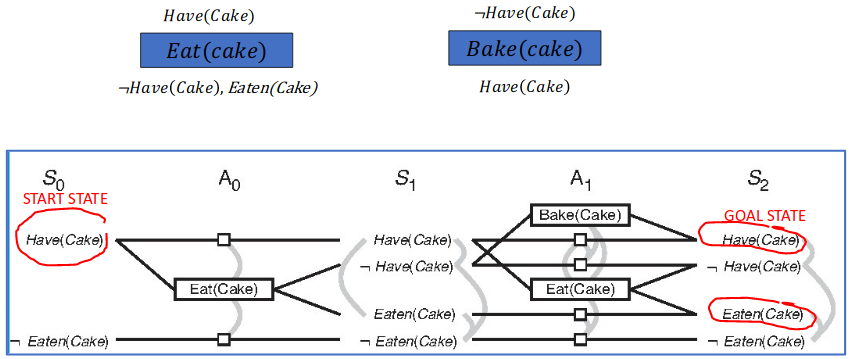
\includegraphics[width=0.9\columnwidth]{img/graph-plan} 
\end{figure}
\begin{itemize}
\item \emph{Level $S_{i}$}: 
\begin{itemize}
\item $i=0$: Start state + literals that could hold at the start. 
\item $i>0$: all literals that could hold at $S_{i}$, depending on actions
at $A_{i-1}$. 
\end{itemize}
\item \emph{Level $A_{i}$}: 
\begin{itemize}
\item Each action in $A_{i}$ connected to its precondition in $S_{i}$
and effect at $S_{i+1}$. 
\item No-op actions: no change. 
\end{itemize}
\item Mutual exclusions between actions when: 
\begin{enumerate}
\item Actions have \emph{inconsistent effects}. 
\item \emph{Interference}: effect of one action = $\lnot$ precondition
of the other. 
\item \emph{Competing needs}: mutually exclusive pre-conditions. 
\end{enumerate}
\item Mutual exclusions between literals when: 
\begin{enumerate}
\item They are \emph{complementary}. 
\item \emph{Inconsistent support}: Each possible pair of actions achieving
them are mutex. 
\end{enumerate}
\item Levels off: when two consecutive levels are identical. 
\end{itemize}

\paragraph{Extracting the Plan}

Once goal is non-mutex in $S_{i}$, search backwards to extract plan.

\section{Knowledge Representation and Automated Reasoning}

\subsection{Intelligent Agents}

An agent that enacts on its environment, based on \emph{observations},
\emph{prior knowledge}, \emph{goals/preferences}, its \emph{abilities}
and sometimes \emph{past experience}.

\begin{figure}[H]
\centering{}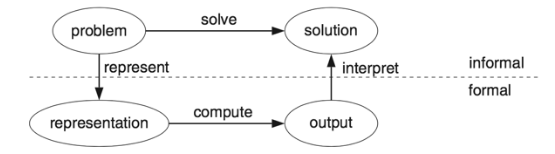
\includegraphics[width=0.6\columnwidth]{img/representation} 
\end{figure}
\begin{enumerate}
\item Find a representation for the problem. 
\item Compute output using automatic reasoning. 
\item Output mapped into solution to the problem. 
\end{enumerate}

\paragraph{Key Decisions}
\begin{enumerate}
\item \emph{Model of the environment}: can be expressed in terms of states
/ features / individuals and relationships between them. 
\item \emph{Uncertainty}: on state (partially observable state) / effects
of actions. 
\item \emph{Preferences}: trade-off between desirability of various outcomes. 
\item \emph{Number of agents}: may be adversarial / cooperative. 
\end{enumerate}

\subsection{Representation}

\paragraph{Representation / Knowledge Schema}

Form of knowledge used in an agent.

\paragraph{Representation}

Internal representation / formalisation of knowledge. Should be: 
\begin{itemize}
\item \emph{Rich enough to express knowledge} needed to solve the problem. 
\item \emph{Close to the problem}: declarative, compact and easy to maintain. 
\item \emph{Amenable to efficient computation}: able to trade of accuracy
and computation time. 
\item \emph{Learnable}: can be automatically acquired from people, past
experience, data. 
\end{itemize}

\paragraph{Knowledge Base}

Representation of all the knowledge that is stored in an agent.

\paragraph{From Problem to Representation}
\begin{itemize}
\item What level of abstraction? 
\begin{itemize}
\item High-level description is harder for a machine to comprehend. May
abstract away important details. 
\item Low-level description can be more accurate and predictive. But more
difficult to reason with \textemdash{} more steps / actions to choose
from. 
\item Multiple levels of abstraction can solve these problems. 
\end{itemize}
\end{itemize}

\paragraph{Solutions}
\begin{itemize}
\item \emph{Optimal}: best solutions according to some criteria. 
\item \emph{Satisficing}: good enough according to some notion of an adequate
solution. 
\item \emph{Approximately optimal}: close enough to the optimal solution. 
\item \emph{Probable}: likely to be a solution. 
\end{itemize}

\subsection{Reasoning}

\paragraph{Reasoning}

Process made by a computational agent when searching for ways to determine
how to complete its task. 
\begin{itemize}
\item \emph{Offline}: background knowledge needed to solve task is precomputed. 
\item \emph{Online}: agents sense the environment to collect and use this
data along with background knowledge, to decide at execution time
what action to take. 
\end{itemize}

\paragraph{Three Forms of Knowledge Inference}
\begin{enumerate}
\item \emph{Deductive}: reasoning from the general to reach the particular
(what necessarily follows from the given?). 
\item \emph{Inductive}: reasoning from the specifics to reach the general
(how can we generalise observations?). 
\item \emph{Abductive}: reasoning from observations to explanations (what
causal relationships are there between knowledge and observations?). 
\end{enumerate}

\subsection{Applying KRR}

\begin{figure}[H]
\centering{}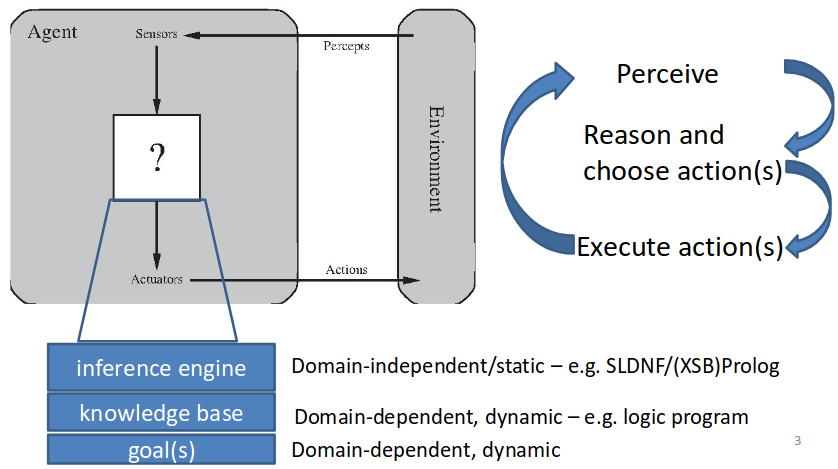
\includegraphics[width=0.75\columnwidth]{img/krr-applications} 
\end{figure}

\paragraph{Ontologies}

Explicit, formal specification of a conceptualisation. 
\begin{itemize}
\item \emph{Concepts of the domain} e.g. classes such as professors, students,
courses. 
\item \emph{Relationships between these terms} e.g. all professors are staff
members. 
\end{itemize}
Allow for a shared understanding of a domain (\emph{semantic interoperability}).

\paragraph{Resource Description Framework (RDF)}

Statements of the form object-attribute-value which assert properties
of objects. 
\begin{itemize}
\item \emph{Triples}: (a, P, b) e.g. (introAI, isTaughtBy, ft). 
\item \emph{Classes}: type(a, C). 
\item \emph{Class hierarchies}: subClassOf(C, D). 
\item \emph{Property hierarchies}: subPropertyOf(P, Q). 
\end{itemize}

\section{Deductive Reasoning}

\paragraph{Clausal Form}

Resolution works with sets / conjunctions of clauses: 
\[
\lnot p_{1}\lor\dots\lor\lnot p_{m}\lor q_{1}\lor\dots\lor q_{n}
\]

where each $p_{i}$ and $q_{j}$ is an atom. 
\begin{itemize}
\item If $m=n=0$: called the empty clause ($\square$). 
\item Every clause can be written as an implication $p_{1}\land\dots\land p_{m}\rightarrow q_{1}\lor\dots\lor q_{n}$. 
\item Every propositional logic formula can be written as a conjunction
of clauses (conjunctive normal form). 
\item Every first-order logic sentence can be written as a conjunction of
clauses (universal qualification + conjunctive normal form + Skolemisation). 
\end{itemize}

\paragraph{Reaching Clausal Form}
\begin{enumerate}
\item Change implication to disjunction: $p\rightarrow q$ goes to $\lnot p\lor q$. 
\item Push negation inwards using: $\lnot\left(p\lor q\right)\equiv\lnot p\land\lnot q$
and $\lnot\left(p\land q\right)\equiv\lnot p\lor\lnot q$. 
\item (First-order) Push negation inwards using $\lnot\exists Xp\left(X\right)\equiv\forall X\lnot p\left(X\right)$
and $\lnot\forall Xp\left(X\right)\equiv\exists X\lnot p\left(X\right)$. 
\item (First-order) Remove existential quantifier in $\exists YF\left[Y\right]$
by: 
\begin{itemize}
\item If the subformula is not in the scope of any universal quantifier,
replace $Y$ with a new Skolem constant: e.g. $\exists Yp\left(Y\right)\implies p\left(c\right)$. 
\item If the subformula occurs in the scope of universal quantifiers for
$X_{1},X_{2},\dots,X_{n}$, replace $Y$ with a new Skolem term $sk\left(X_{1},X_{2},\dots X_{n}\right)$:
e.g. $\forall X\exists Yp\left(X,Y\right)\implies p\left(X,f\left(X\right)\right)$. 
\end{itemize}
\item (First-order) Move all universal quantifiers to the front of the sentence
using: $\forall X\varphi_{1}\left(X\right)\land\varphi_{2}$ is equivalent
to $\forall X\left(\varphi_{1}\left(X\right)\land\varphi_{2}\right)$
after appropriately renaming variables if $X$ occurs in $\varphi_{2}$. 
\item Distribute $\lor$ over $\land$ using: $p\lor\left(q\land s\right)\equiv\left(p\lor q\right)\land\left(p\lor s\right)$. 
\end{enumerate}

\subsection{Unification}

\paragraph{Universal Instantiation}

Combines two clauses: 
\[
\dfrac{\forall v\alpha}{\alpha\left\{ v/g\right\} }\qquad\text{(for Alessandra: \ensuremath{\left\{ v=g\right\} )}}
\]
for any variable $v$ and term $g$. 
\begin{itemize}
\item $\sigma=\left\{ v/g\right\} $ is a \emph{substitution}. $\alpha\sigma$
means the formula obtained from $\alpha$ by applying $\sigma$. 
\item $a'$ is an \emph{instance} of $a$ if $a=a\sigma$ for some $\sigma$. 
\end{itemize}

\paragraph{Unification}

A substitution $\sigma$ unifies atomic sentences $p$ and $q$ if
$p\sigma=q\sigma$. 
\begin{itemize}
\item E.g. $p=\text{Knows}\left(\text{John},x\right)$, $\text{Knows}\left(y,\text{OJ}\right)$,
$\sigma=\left\{ x/\text{OJ},y/\text{John}\right\} $. 
\end{itemize}

\paragraph{Most General Unifier}

$\theta$ is a most general unifier of formulas $\alpha$ and $\beta$
if: 
\begin{enumerate}
\item $\theta$ unifies formulas $\alpha$ and $\beta$. 
\item If $\sigma$ is any other unifier of $\alpha$ and $\beta$, then
$\alpha\sigma$ is an instance of $\alpha\theta$ (i.e. $\alpha\sigma=\left(\alpha\theta\right)\sigma'$
for some $\sigma'$). 
\end{enumerate}

\subsection{Resolution}

\subsubsection{Propositional Logic}

\paragraph{Resolution Inference Rule}

Combines two clauses: 
\[
\dfrac{\alpha\lor\beta,\lnot\beta\lor\gamma}{\alpha\lor\gamma}
\]

Applied repeatedly until $\square$ is derived.

\paragraph{Soundness of Resolution}

If $S\vdash P$ by resolution, then $S\vDash P$.

\paragraph{Refutation Completeness of Resolution}
\begin{itemize}
\item If conjunction of propositional clauses is unjustifiable, we will
end up with $\square$. 
\item To prove a goal $P$ is entailed by a set of sentences $S$ ($S\vDash P$): 
\begin{enumerate}
\item Compute CNF of $S$ and $\lnot P$. 
\item Apply resolution to results of step 1 to obtain $\square$. 
\end{enumerate}
\end{itemize}

\subsubsection{First-Order Logic}

\paragraph{Resolution Inference Rule}

For proof by resolution, draw a tree.

\[
\dfrac{\alpha\lor\beta,\lnot\beta'\lor\gamma}{\left(\alpha\lor\gamma\right)\theta}\text{ where \ensuremath{\theta} is a mgu of \ensuremath{\beta} and \ensuremath{\beta'}}
\]

after appropriately renaming variables to be distinct. Full version:
\[
\dfrac{\alpha^{1}\lor\dots\lor a^{j-1}\lor a^{j}\lor a^{j+1}\lor\dots\lor\alpha^{m},\beta^{1}\lor\dots\lor\beta^{k-1}\lor\beta^{k}\lor\beta^{k+1}\lor\dots\lor\beta^{n}}{\left(\alpha^{1}\lor\dots\lor a^{j-1}\lor a^{j+1}\lor\dots\lor\alpha^{m},\beta^{1}\lor\dots\lor\beta^{k-1}\lor\beta^{k+1}\lor\dots\lor\beta^{n}\right)\theta}
\]
where $\theta$ is a mgu of $\alpha^{j}$ and $\lnot\beta^{k}$.

\subsubsection{Generalised Modus Ponens 
\[
\dfrac{p'_{1},p'_{2},\dots,p'_{n},\left(q\leftarrow p_{1},p_{2},\dots,p_{n}\right)}{q\theta}
\]
}

where $p'_{i}\theta=p_{i}\theta$.

\subsection{SLD Resolution}

\paragraph{Definite Clauses}

Clauses of the form (for atoms $p,q_{1},\dots,q_{n}$) 
\[
p\leftarrow q_{1},q_{2},\dots,q_{n}
\]
\begin{itemize}
\item $p$ is the \emph{head} and $q_{1},\dots,q_{n}$ the \emph{body} of
the clause. 
\item If $n=0$, $p$ is a \emph{fact}. 
\item A set of definite clauses is a \emph{logic program} / \emph{knowledge
base}. 
\item A \emph{Horn clause} / \emph{denial} is a definite clause or $\leftarrow q_{1},\dots,q_{n}$. 
\end{itemize}

\paragraph{SLD Resolution}

Linear Resolution for Definite clauses with Selection function

\[
\dfrac{\overbrace{\lnot\alpha^{1}\lor\dots\lor\lnot\alpha^{j}\lor\dots\lor\lnot\alpha^{m}}^{\text{Goal (denial)}},\overbrace{\alpha\lor\lnot\beta^{1}\lor\dots\lor\lnot\beta^{n}}^{\text{Definite Clause}}}{\left(\lnot\alpha^{1}\lor\dots\lor\lnot\beta^{1}\lor\dots\lor\lnot\beta^{n}\lor\dots\lor\lnot a^{m}\right)\theta}
\]
where $\theta$ is a mgu of $\alpha^{j}$ and $\alpha$.

\paragraph{Alternative View SLD Resolution}

\begin{align*}
\: & \leftarrow L_{1},\dots,L_{j-1},B,L_{j+1},\dots,L_{n}\\
\theta_{i} & \mid\text{match \ensuremath{B} with \ensuremath{B'\leftarrow M_{1},\dots,M_{k}} since \ensuremath{B\theta_{i}=B'\theta_{i}}}\\
\: & \leftarrow\left(L_{1},\dots,L_{j-1},M_{1},\dots,M_{k},L_{j+1},\dots,L_{n}\right)\theta_{i}
\end{align*}
\begin{itemize}
\item Answer is computed from composition of all mgus. 
\item Sub-goal $B$ can be chosen in any way. 
\item There may be many choices for the matching clause. Forms a SLD tree. 
\end{itemize}

\subsection{Forward and Backward Chaining}

To prove that $S\vDash P$: 
\begin{enumerate}
\item Compute the CNF $S'$ of $S$. 
\item Compute the CNF $NP'$ of $\lnot P$. 
\item If $S'$ is a set of definite clauses (logic program) and $NP'$ is
a Horn clause $\leftarrow q_{1},\dots,q_{n}$, then apply GMP to derive
$q_{1},\dots,q_{n}$ from $S'$. 
\end{enumerate}

\paragraph{Forward Chaining (Bottom-Up Computation)}
\begin{enumerate}
\item Split $S'$ into facts $E$ and definite clauses (rules) $Pr$. 
\item Apply the rules in $Pr$ to the facts in $E$ using GMP to derive
implied facts $E'$. 
\item Add $E'$ to $E$. 
\item Repeat until no new facts are generated. 
\item Succeed iff $q_{1},\dots,q_{n}$ are in $E$. 
\end{enumerate}
Likely to produce a lot of irrelevant facts.

\paragraph{Backward Chaining (Top-Down / Goal-Directed Computation)}

Start with goals $q_{1},\dots,q_{n}$ and $\theta=\{\}$. To solve
a goal $G$ wrt $\theta$: 
\begin{enumerate}
\item If there is a matching fact $G'$ in $S'$, add mgu $\sigma$ to $\theta$
($G\sigma=G'\sigma$). 
\item For each rule $G'\leftarrow G_{1},\dots,G_{m}$ in $S'$ whose head
$G'$ matches $G$ via mgu $\sigma'$, solve goals $G_{1}\sigma',\dots,G_{m}\sigma'$
wrt to $\theta+\left\{ \sigma'\right\} $. 
\item Repeat until there are no goals to solve, return $\theta$. 
\end{enumerate}

\subsection{Semantics of Definite Clauses}
\begin{itemize}
\item \emph{Herbrand universe}: set of all ground terms that can be constructed
from constant and function symbols in $S$. 
\item Each set of definite clauses $S$ can be can be equated to the set
of all its ground instances over the underlying Herbrand universe. 
\end{itemize}

\paragraph{Classical Models}

Interpretations of $S$: 
\begin{itemize}
\item Mappings from ground terms of $S$ to elements of some domain $D$. 
\end{itemize}
Models of $S$: 
\begin{itemize}
\item Interpretations of $S$ in which every clause of $S$ is true. 
\end{itemize}

\paragraph{Herbrand Models}

Models where ground terms denote themselves (i.e. domain is Herbrand
universe of $S$). 
\begin{itemize}
\item $S$ has a model iff $S$ has a (minimal) Herbrand model. 
\end{itemize}

\paragraph{Immediate Consequence Operator $T_{s}$}
\begin{itemize}
\item \emph{Herbrand Base} $HB$: Set of all ground atoms constructed from
predicate symbols in $S$ over the Herbrand universe of $S$. 
\item Given $X\subseteq HB$, $T_{s}\left(X\right)=\left\{ a\in HB\mid a\leftarrow b_{1},\dots,b_{m}\in S,\left\{ b_{1},\dots,b_{m}\right\} \subseteq X\right\} $. 
\item Least fixed point, given by $T_{s}\uparrow^{\omega}=\cup_{i=0}^{\infty}T_{s}\left(\emptyset\right)$,
which is the minimal Herbrand model of S. 
\end{itemize}

\subsection{SLD Resolution is Complete}

If $S\vDash P\sigma$ (i.e. $P\sigma$ belongs to the minimal Herbrand
model of $S$), then there exists and SLD-refutation of $P$ to obtain
$\square$ with answer $\theta$ and a substitution of $\xi$ such
that $P\sigma=P\theta\xi$.

\subparagraph{Example}

\begin{align*}
 & S=\left\{ P\left(x,y\right)\leftarrow Q\left(x\right),Q\left(1\right)\leftarrow,R\left(2\right)\leftarrow\right\} \\
 & \leftarrow P\left(x,y\right)\\
 & \leftarrow Q\left(x\right)\\
 & \square\theta=\left\{ x/1\right\} 
\end{align*}

$P\left(1,2\right)$ belongs to the minimal Herbrand model of $S=\left\{ Q\left(1\right),R\left(2\right),P\left(1,1\right),P\left(1,2\right)\right\} $
with $\xi=\left\{ y/2\right\} $.

\section{Deductive Reasoning with NAF}

\subsection{Non-monotonic Reasoning}

\paragraph{Non-monotonic Logics}

Conclusions can be invalidated by adding more knowledge.

\paragraph{Default Reasoning}

In the absence of information to the contrary, results follow by default.

E.g. 
\begin{align*}
 & \text{BIRDS}=\text{flies}\left(X\right)\leftarrow,\lnot\text{penguin}\left(X\right),\lnot\text{wounded}\left(X\right),\dots\\
 & \text{BIRDS}\cup\left\{ \text{bird}\left(\text{tweety}\right)\right\} \vDash^{*}\text{flies}\left(\text{tweety}\right)\\
 & \text{BIRDS}\cup\left\{ \text{bird}\left(\text{tweety}\right)\right\} \cup\left\{ \text{penguin}\left(\text{tweety}\right)\right\} \not\vDash^{*}\text{flies}\left(\text{tweety}\right)
\end{align*}

\paragraph{Closed World Assumption}

If $\alpha$ is not present in some $DB$, then assume $\lnot\alpha$.

\paragraph{Negation as Failure}

$\lnot B$ succeeds when all attempts to prove $B$ fail (finitely).

\paragraph{Credulous vs. Sceptical Reasoning}

Assume Quakers are pacifists and republicans are not. Nixon is a Quaker
and a Republican. Is Nixon a pacifist or not? 
\begin{itemize}
\item \emph{Sceptical / cautious reasoning}: No. 
\item \emph{Credulous / brave reasoning}: Yes, to both. 
\end{itemize}

\subsection{SLDNF}

Derivation steps: 
\begin{itemize}
\item Select any positive literal $L_{j}=B$ from the current goal: 
\end{itemize}
\begin{align*}
\: & \leftarrow L_{1},\dots,L_{j-1},B,L_{j+1},\dots,L_{n}\\
\theta_{i} & \mid\text{match \ensuremath{B} with \ensuremath{B'\leftarrow M_{1},\dots,M_{k}} since \ensuremath{B\theta_{i}=B'\theta_{i}}}\\
\: & \leftarrow\left(L_{1},\dots,L_{j-1},M_{1},\dots,M_{k},L_{j+1},\dots,L_{n}\right)\theta_{i}
\end{align*}
\begin{itemize}
\item Select any (\emph{safe} / \emph{ground} - otherwise will \emph{flounder})
negative literal $L_{j}=\text{not }B$ from the current goal: 
\end{itemize}
\begin{align*}
\: & \leftarrow L_{1},\dots,L_{j-1},\text{not }B,L_{j+1},\dots,L_{n}\\
\theta_{i}=\{\} & \mid\text{all ways of computing goal \ensuremath{B} must fail (finitely)}\\
\: & \leftarrow\left(L_{1},\dots,L_{j-1},L_{j+1},\dots,L_{n}\right)\theta_{i}
\end{align*}

\paragraph{Properties}

Consider 
\begin{align*}
 & p\left(X\right)\leftarrow q\left(X\right),\text{not }r\left(X\right)\\
 & q\left(a\right)\\
 & r\left(b\right)
\end{align*}
\begin{itemize}
\item \emph{Non-monotonic}: $S\vdash_{\text{SLDNF}}p\left(a\right)$ but
$S\cup\left\{ r\left(a\right)\right\} \not\vdash_{\text{SLDNF}}p\left(a\right)$. 
\item Builds in a kind of \emph{CWA}: $S\cup\left\{ r\left(a\right)\right\} \vdash_{\text{SLDNF}}\lnot p\left(a\right)$. 
\end{itemize}

\subsection{Semantics for Normal Logic Programs}

\subsubsection{(Clark) Completion Semantics}

The \emph{completion} of $S$ is found by: 
\begin{enumerate}
\item Rewrite all rules in $S$ as rules of the form 
\[
p\left(\overrightarrow{X}\right)\leftarrow\overrightarrow{X}=\overrightarrow{t},\text{body}
\]
so $p\left(X,3\right)\leftarrow q\left(X\right),\text{not }r\left(3\right)$
becomes $p\left(X,Y\right)\leftarrow Y=3\land q\left(X\right)\land\lnot r\left(3\right)$ 
\item Combine all rules with the same head so 
\[
p\left(\overrightarrow{X}\right)\leftarrow\overrightarrow{X}=\overrightarrow{t}_{1},\text{body}_{1},\dots,p\left(\overrightarrow{X}\right)\leftarrow\overrightarrow{X}=\overrightarrow{t}_{n},\text{body}_{n}
\]
becomes 
\[
p\left(\overrightarrow{X}\right)\leftrightarrow\overrightarrow{X}=\overrightarrow{t}_{1},\text{body}_{1}\lor\dots\lor p\left(\overrightarrow{X}\right)\leftarrow\overrightarrow{X}=\overrightarrow{t}_{n},\text{body}_{n}
\]
\item If some $q\left(\underline{\;}\right)$ is not the head of any rule
in $S$, add $q\left(\overrightarrow{X}\right)\leftrightarrow\text{false}$. 
\item Add Clark's Equality Theory: 
\begin{enumerate}
\item $f\left(\overrightarrow{t}\right)\neq g\left(\overrightarrow{s}\right)$
for all pairs of distinct terms in the Herbrand universe of $S$. 
\item $X=X,X=Y\rightarrow Y=X,X=Y\land Y=Z\rightarrow X=Z$. 
\item $\overrightarrow{X}=\overrightarrow{Y}\rightarrow p\left(\overrightarrow{X}\right)=p\left(\overrightarrow{Y}\right)$
for all predicate symbols $p$ in $S$. 
\item $\overrightarrow{X}\neq t\left[\overrightarrow{X}\right]$ for all
terms $t$ where $\overrightarrow{X}$ occurs. 
\end{enumerate}
\end{enumerate}

\paragraph{Soundness of SLDNF}
\begin{itemize}
\item If there is a SLDNF-refutation of $P$ from $S$ with answer $\theta$
then $\text{Completion}\left(S\right)\vDash P\theta$. 
\item If there is a \emph{finitely-failed} SLDNF-refutation of $P$ from
$S$ then $\text{Completion}\left(S\right)\vDash\lnot P$. 
\end{itemize}

\subsubsection{Well-Founded Model Semantics}

$\left(\text{In},\text{Out}\right)$ such that: 
\begin{enumerate}
\item $\text{In}\subseteq HB$. 
\item $\text{Out}\subseteq HB^{\text{not}}=\left\{ \text{not }a\mid a\in HB\right\} $ 
\end{enumerate}
\rule[0.5ex]{0.25\columnwidth}{0.5pt} 
\begin{itemize}
\item Atoms in $HB-\left(\text{In}\cup\left\{ a\mid\text{not }a\in\text{Out}\right\} \right)$
are `undecided'. 
\item For $S=\left\{ p\leftarrow\text{not }p\right\} $, the well-founded
model is $\left(\{\},\{\}\right)$ so $p$ is undecided. 
\end{itemize}

\subsubsection{Stable Model Semantics}

Given a normal logic program $S$ and $X\subseteq HB$, the reduce
of $S$ by $X$, $S^{X}$ is obtained by: 
\begin{enumerate}
\item Eliminate all rules with $\text{not }p$ in the body, for every $p\in X$. 
\item Eliminate all negative literals from the body of all remaining rules. 
\end{enumerate}
$X\subseteq HB$ is a \emph{stable model} of $S$ iff the least Herbrand
model of $S^{X}$ is $X$. 
\begin{itemize}
\item \emph{Credulous reasoning}: whatever holds in some stable model. 
\item \emph{Sceptical reasoning}: whatever holds in all stable models. 
\end{itemize}

\section{Abductive Reasoning}

$\left(KB,A,IC\right)$ is an \emph{abductive logic program} where: 
\begin{itemize}
\item $KB$ is the theory (a set of normal clauses). 
\item $A$ is the set of aducibles in $BK$ (ground \emph{undefined} literals). 
\item $IC$ is a set of integrity constraints (denials - must be false). 
\item $G$ is the goal / observation. 
\end{itemize}

\paragraph{Properties of Explanations}

An \emph{abductive solution} is a set $\Delta$ of ground literals
that are: 
\begin{enumerate}
\item \emph{Basic}: should be restricted to \emph{aducibles} (ground literals
with predicates that are not defined in the theory). 
\item \emph{Minimal}: should not be subsumed by other explanations. 
\item \emph{Consistent}: with the given theory, including integrity constraints. 
\end{enumerate}
Formally: 
\begin{enumerate}
\item $\Delta\subseteq A$: belongs to aducibles. 
\item $KB\cup\Delta\vDash G$: provides missing information needed to solve
goal. 
\item $KB\cup\Delta\not\vDash\bot$: consistent with knowledge base. 
\item $KB\cup\Delta\vDash IC$: satisfies integrity constraints. 
\end{enumerate}

\subsection{Abduction by Extending SLDNF}

\paragraph{Abductive Derivation}
\begin{itemize}
\item Perform SLDNF but maintain an accumulator $\Delta$ to which unproved
sub-goals are added as assumptions. 
\item Order in which literals appear in a clause only influences order in
which aducibles are added to explanation (not the explanation itself). 
\end{itemize}

\paragraph{Consistency Derivation (Special Cases)}
\begin{itemize}
\item \emph{Integrity constraints}: making an assumption on aducibles in
integrity constraints requires checking the satisfiability of these
integrity constraints. 
\begin{itemize}
\item Resolve assumed literal with all relevant integrity constraints and
ensure it fails. 
\end{itemize}
\item \emph{Negation as failure}: requires adding a consistency phase: look
for explanations, in terms of aducibles, for failure. 
\begin{itemize}
\item Implicitly add all negative literals to $A$. 
\item Implicitly add $\leftarrow P,\text{not }P$ to $IC$ for all predicates
$P$. 
\end{itemize}
\end{itemize}

\subsection{Operational Semantics of Abduction}

\begin{figure}[H]
\centering{}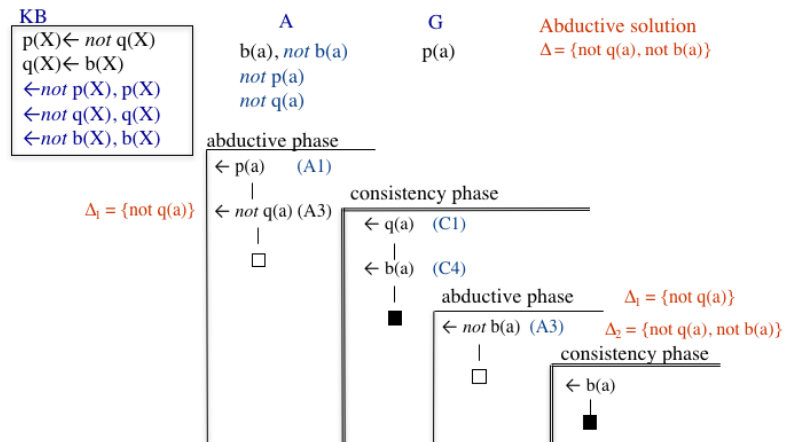
\includegraphics[width=0.75\columnwidth]{img/abduction-example} 
\end{figure}

\paragraph{Abductive Phase}

Consider each literal in the goal, left to right. Start with an abductive
phase. 
\begin{enumerate}
\item \emph{The current goal is not an aducible}. Initiate SLDNF derivation
with current goal to be proved by refutation. If literal is positive,
use normal resolution, otherwise go to case 3. 
\item \emph{The current goal is an aducible}. If the goal is already part
of $\Delta$, then the resolution is already proved and we proceed
to the next goal. 
\item \emph{The current goal is an aducible not yet assumed}. Assume the
literal. Trigger a consistency phase (failure derivation). If it does
derive a failure, continue with the updated $\Delta$. 
\end{enumerate}

\paragraph{Consistency Phase}

In the consistency phase, consider each literal from each constraint
(denial) which includes the assumed literal. 
\begin{enumerate}
\item \emph{The literal is not an aducible}. Then apply a SLDNF failure
derivation of this literal. 
\item \emph{The literal is already assumed in} $\Delta$. This literal succeeds,
so we need to check the rest to prove that it fails. 
\item \emph{The literal's negation is already assumed in} $\Delta$. This
literal fails, and so the current constraint is satisfied. Continue
to the next constraint. 
\item \emph{Otherwise}. Trigger an abductive derivation of this literal's
negation. If it succeeds, then this constraint is satisfied. Continue
to the next constraint with the updated $\Delta$. 
\end{enumerate}

\subsection{Semantic Properties of Abduction}

\paragraph{Knowledge Assimilation}

Explanation of new information computed abductively and added to $KB$.

\paragraph{Non-Monotonicity}

Use abduction for default reasoning. E.g. suppose $\text{fly}\left(X\right)\leftarrow\text{bird}\left(X\right)$
by default, but $\text{bird}\left(X\right)\leftarrow\text{penguin}\left(X\right)$
and $\lnot\text{fly}\left(X\right)\leftarrow\text{penguin}\left(X\right)$:

\begin{align*}
KB & \begin{cases}
\text{bird}\left(X\right)\leftarrow\text{penguin}\left(X\right)\\
\text{not\_fly}\left(X\right)\leftarrow\text{penguin}\left(X\right)\\
\text{fly}\left(X\right)\leftarrow\text{bird}\left(X\right),\text{birdsFly}\left(X\right)
\end{cases}\\
IC & \leftarrow\text{birdsFly}\left(X\right),\text{not\_fly}\left(X\right)
\end{align*}

Or using NAF:

\begin{align*}
KB & \begin{cases}
\text{bird}\left(X\right)\leftarrow\text{penguin}\left(X\right)\\
\text{abnormal}\left(X\right)\leftarrow\text{penguin}\left(X\right)\\
\text{fly}\left(X\right)\leftarrow\text{bird}\left(X\right),\text{not abnormal}\left(X\right)
\end{cases}\\
IC & \emptyset\text{ (\ensuremath{\rightarrow\text{abnormal}\left(X\right),\text{not abnormal}\left(X\right)} implicitly)}
\end{align*}

I.e. $KB\vdash Q$ under SLDNF if $Q$ has an abductive solution after: 
\begin{enumerate}
\item Renaming all uses of $\text{not }q\left(X\right)$ to $q*\left(X\right)$. 
\item Adding $q*\left(X\right),q\left(X\right)$ to $IC$. 
\end{enumerate}

\subsection{Applications of Abduction}
\begin{itemize}
\item Diagnosis Problems 
\item Planning 
\end{itemize}

\paragraph{Event Calculus}

Logical framework for representing and reasoning about events and
effects over time. 
\begin{itemize}
\item \emph{Ontology} consists of events, fluents and time. 
\item \emph{Signature} includes: 
\begin{itemize}
\item $\text{initiates}(e,f,t)$: Fluent $f$ starts to hold after event
$e$ at time $t$. 
\item $\text{terminates}(e,f,t)$: Fluent $f$ stops holding after event
$e$ at time $t$. 
\item $\text{initially}(f)$: Fluent $f$ holds at the beginning. 
\item $\text{happens}(e,t)$: Event $e$ happens at time $t$. 
\item $\text{holdsAt}(f,t)$: Fluent $f$ holds at time $t$. 
\item $\text{clipped}(t_{1},f,t_{2})$: Fluent $f$ is terminated between
times $t_{1}$ and $t_{2}$. 
\end{itemize}
\end{itemize}
Description includes two theories: 
\begin{itemize}
\item \emph{Domain independent theory}: General rules for when fluents hold
at certain times. 
\begin{itemize}
\item $\text{holdsAt}\left(f,t_{2}\right)\leftarrow\text{initially}\left(f\right),\text{not clipped}\left(0,f,t_{2}\right)$:
initially true fluents hold until an event terminates them. 
\item $\text{holdsAt}\left(f,t_{2}\right)\leftarrow\text{initiates}\left(e,f,t_{1}\right),\text{happens}\left(e,t_{1}\right),t1<t2,\text{not clipped}\left(t_{1},f,t_{2}\right)$:
fluents initiated by an event hold until an event terminates them. 
\item $\text{clipped}\left(t_{1},f,t\right)\leftarrow\text{happens}\left(e,t_{2}\right),\text{terminates}\left(e,f,t_{2}\right),t_{1}<t_{2},t_{2}<t$:
fluents only change status via terminating events. 
\end{itemize}
\item \emph{Domain dependent theory}: Particular effects of events or actions,
using $\text{initiates}(.)\leftarrow\text{BODY}$ and $\text{terminates}(.)\leftarrow\text{BODY}$,
as well as initial state (using $\text{initially}(.)$) and event
occurrences (using $\text{happens}(.)$). 
\begin{itemize}
\item Preconditions are captured in the conditions in initiates axioms. 
\item Effects are expressed by head atoms of initiates and terminates rules. 
\end{itemize}
\end{itemize}

\paragraph{Event Calculus Abductive Planning}

Given 
\begin{itemize}
\item $DI$: domain independent theory. 
\item $DD$: domain dependent theory. 
\item $A$: set of ground aducibles.
\item $IC$: integrity constraints (usually $\left\{ \text{happens}\left(E_{1},T\right),\text{happens}\left(E_{2},T\right),E_{1}\neq E_{2}\right\} $). 
\item $G$: goal state. 
\end{itemize}
A plan is some $P=\left(As,TC\right)$ where 
\begin{itemize}
\item $As=\left\{ \text{happens}\left(e_{i},t_{i}\right),\text{happens}\left(e_{j},t_{j}\right),\dots\right\} $. 
\item $TC=\left\{ t_{i}<t_{j},\dots\right\} $. 
\end{itemize}
such that 
\begin{itemize}
\item $DI\cup DD\cup P\vDash G$. 
\item $DI\cup DD\cup P\cup IC$ is consistent. 
\end{itemize}
Setting $KB=DI\cup DD$ and $\Delta=P$: 
\begin{itemize}
\item $KB\cup\Delta\vDash G$. 
\item $KB\cup\Delta\cup IC\not\vDash\bot$. 
\end{itemize}

\section{SAT Solving}

Given a propositional formula $\varphi$ (usually in CNF), SAT on
$\varphi$ means to determine if there exists a variable assignment
under which $\varphi$ evaluates to true.

\paragraph{Why CNF?}
\begin{itemize}
\item Efficient algorithms to transform formulae into CNF. 
\item Can exploit CNF: easier to detect conflicts. 
\end{itemize}

\paragraph{SAT Algorithms}
\begin{itemize}
\item Complete algorithms: 
\begin{itemize}
\item \emph{Proof systems}: e.g. truth table / natural deduction. 
\item \emph{Davis-Putman} (DP): based on resolution. 
\item \emph{Stalmark's method}. 
\item \emph{Davis-Logemann-Loveland} (DLL/DPLL): search-based. 
\item \emph{Conflict-Driven Clause Learning} (CDCL). 
\end{itemize}
\item Incomplete algorithms: 
\begin{itemize}
\item Local search / hill climbing. 
\item Genetic algorithms. 
\end{itemize}
\end{itemize}

\subsection{DP Algorithm}

For a set $S$ of clauses, for each variable in $S$: 
\begin{enumerate}
\item For each clause $C_{i}$ containing the variable and each clause $C_{j}$
containing its negation, resolve $C_{i}$ and $C_{j}$. (Fail if resolvent
is $\square$). 
\item Add the resolvent to $S$. 
\item Remove $S$ from all clauses. 
\end{enumerate}
Final set of variables informs a \emph{partial assignment}.

\paragraph{Improvements}
\begin{itemize}
\item Ignore when resolution generates a tautology (literal and its negation). 
\item \textbf{Pure literal rule} 
\begin{itemize}
\item \emph{Pure literal}: only ever occurs with the same polarity. 
\item Clauses containing pure literals can be removed. 
\item Remember required assignments. 
\end{itemize}
\item \textbf{Unit propagation rule} 
\begin{itemize}
\item \emph{Unit clause}: clause with a single literal. 
\item Satisfy the literal by making it true. 
\item Propagate the assignment by removing clauses that contain the literal,
and removing the negated literal from any clauses that contain it. 
\end{itemize}
\end{itemize}

\subsection{DLL Algorithm}

\paragraph{Key Idea}

Instead of eliminating variables, split on a variable at each step.

\paragraph{Simplifications}

Given a set $Sc$ of clauses: 
\begin{itemize}
\item $\text{UNSAT}\left(Sc\right)$: if $Sc$ contains $\{\}$ then formula
is unsatisfiable. 
\item $\text{SAT}\left(Sc\right)$: if $Sc=\{\}$ then formula is satisfiable. 
\item $\text{MULT}\left(L,Sc\right)$: if literal occurs more than once
in a clause in $Sc$, all but one can be deleted. 
\item $\text{SUB}\left(C,Sc\right)$: A clause in $Sc$ can be deleted if
it is a superset of another clause in $Sc$. 
\item $\text{TAUT}\left(C,Sc\right)$; A clause in $Sc$ that contains a
literal and its negation can be deleted. 
\item $\text{PURE}\left(L,Sc\right)$: If $L$ is a pure literal in $Sc$,
delete all clauses containing $L$ and add $L$ to the assignment. 
\item $\text{UNIT}\left(L,Sc\right)$: If $Sc$ contains a unit clause $\{L\}$,
delete all clauses including $L$, remove $\lnot L$ from the remaining
clauses, and add $L$ to the assignment. 
\item $\text{SPLIT}\left(L,Sc\right)$: If $Sc$ contains clauses of the
from $\left\{ C_{k},L\right\} $ and $\left\{ C_{m},\lnot L\right\} $,
branch the computation (adding $L$ and $\lnot L$ to each branch's
assignment respectively), and regenerate $Sc$ using the UNIT rule. 
\end{itemize}

\section{Answer Set Programming}

\subsection{Semantics}

All rules must be safe: 
\begin{itemize}
\item A rule $R$ is safe, if every variable in $R$ occurs in $\text{body}^{+}\left(R\right)$. 
\end{itemize}
To check with $X$ is an answer set of a program $P$: 
\begin{enumerate}
\item Find the \emph{relevant grounding} $\mathcal{RG}\left(P\right)$: 
\begin{enumerate}
\item For each rule $R$ in $P$, generate all rules which are ground instances
$R_{g}$ of $R$, s.t. for each atom $A$ in $\text{body}^{+}\left(R_{g}\right)$
there is at least one rule already in $\mathcal{RG}\left(P\right)$
with $A$ as the head. 
\end{enumerate}
\item Calculate the reduct of $\mathcal{RG}\left(P\right)$ w.r.t. $X$,
$\mathcal{RG}\left(P\right)^{X}$: 
\begin{enumerate}
\item Remove any rule whose body contains the negation of an atom in $X$. 
\item Delete any negation from the remaining rules. 
\end{enumerate}
\item Check whether $X=M\left(\mathcal{RG}\left(P\right)^{X}\right)$ (the
LHM of the reduct). 
\begin{enumerate}
\item Find LHM by starting with $M=\{\}$ iteratively adding any atom that
is the head of a rule in $P$ whose body is already satisfied by $M$. 
\end{enumerate}
\end{enumerate}

\paragraph{Relationship between ASP and Clark Completion}

The answer sets of $P$ are the models of $\text{completion}$$\left(P\right)$
which have no non-empty unfounded subsets w.r.t. $P$. 
\begin{itemize}
\item Given an interpretation $I$, $U\subseteq I$ is an \emph{unfounded
subset} w.r.t. $P$ if there's no rule $R$ in $P$ that proves anything
in $U$ without using elements of $U$. I.e. no rule s.t.: 
\begin{enumerate}
\item $I$ satisfies $\text{body}\left(R\right)$. 
\item $\text{head}\left(R\right)\in U$. 
\item $I\cap\text{body}^{+}\left(R\right)=\emptyset$. 
\end{enumerate}
\end{itemize}

\paragraph{Brave and Cautious Semantics}
\begin{itemize}
\item $P$ \emph{bravely} entails $A$ if \emph{some} answer set of $P$
contains $A$. 
\item $P$ \emph{cautiously} entails $A$ if \emph{every} answer set of
$P$ contains $A$. 
\end{itemize}

\subsection{Constraints}

\paragraph{Choice Rules}

If the body is satisfied by an answer set, then the number of $h_{i}$s
should be between $\mathtt{lb}$ and $\mathtt{ub}$.

\[
\mathtt{lb}\left\{ h_{1};\dots;h_{m}\right\} \mathtt{ub}\;:-\;b_{1},\dots,b_{n}
\]

Now when constructing the reduct: 
\begin{itemize}
\item If $X$ satisfies the head of $R$, then for each atom $h$ that occurs
both in the head and in $X$, $P^{X}$ contains $h\::-\;\text{body}^{+}\left(R\right)$. 
\item If $X$ doesn't satisfy the head of $R$, then $P^{X}$ contains $:-\;\text{body}^{+}\left(R\right)$. 
\end{itemize}
Choice rules can generate non-minimal answer sets.

\paragraph{Disjunction}

Represented using $;$. Unlike choice sets, all answer sets are minimal
models.

\paragraph{Hard Constraints}

Eliminates any answer that satisfies $b_{1}\land\dots\land b_{n}$.

\[
:-\;b_{1},\dots,b_{n}
\]

\paragraph{Abduction in ASP}

Rewrite the aducibles as a choice rule, and the goal as a constraint.

\subsection{Aggregates}

\[
\mathtt{lb\#agg}\left\{ e_{1};\dots;e_{n}\right\} \mathtt{ub}
\]

is satisfied by $X$ iff 
\[
\mathtt{lb\#agg}\left(\mathrm{eval}\left(X,\left\{ e_{1},\dots,e_{n}\right\} \right)\right)\mathtt{ub}
\]
\begin{itemize}
\item Variables which only occur inside aggregates are \emph{local}, and
produce multiple aggregate elements, instead of multiple rules. 
\begin{itemize}
\item \emph{Safety}: a rule with an aggregate is unsafe if a local variable
occurs in an aggregate element but doesn't occur in a positive literal
on the RHS of the element. 
\end{itemize}
\item Semantics usually defined by $FLP$ reduct. 
\[
P_{FLP}^{X}=\left\{ r\in P\mid X\vDash\text{body}\left(I\right)\right\} 
\]
but this doesn't always have a minimal model. 
\end{itemize}

\subsection{Optimisation}

\paragraph{Weak Constraints}

\[
:\sim\:b_{1},\dots,b_{m}.\left[\mathtt{wt@lev},t_{1},\dots,t_{n}\right]
\]

The score at a priority level $p$ is 
\[
\text{score}\left(P,p,X\right)=\sum\mathtt{wt}.\left[\mathtt{wt@p},t_{1},\dots,t_{n}\right]_{\in\text{Weak}\left(P,X\right)}
\]
\begin{itemize}
\item $X_{1}$ is preferred to $X_{2}$ if for the highest priority where
their scores differ, $X_{1}$ has a lower score. 
\end{itemize}

\end{document}
